\documentclass[aspectratio=149]{beamer}
\usepackage[english]{babel}
\usepackage[utf8x]{inputenc}
\usepackage{amsmath, amsthm}
\usepackage{amssymb}
\usepackage{tikz}
\usetikzlibrary{calc,shapes,positioning, arrows.meta}
\usepackage{graphicx, subfig}
%\usepackage[ruled,linesnumbered]{algorithm2e}

%\renewcommand{\bibsection}{}
%\newcommand{\tikzmark}[1]{\tikz[overlay,remember picture] \node (#1) {};}

%%algorithm
%\let\oldnl\nl% Store \nl in \oldnl
%\newcommand{\nonl}{\renewcommand{\nl}{\let\nl\oldnl}}% Remove line number for one line
%% new colour
%\definecolor{darkcerulean}{rgb}{0.03, 0.27, 0.49}
%% underbrace with normal font
%\newcommand{\bunderbrace}[2]{%
%  \begin{array}[t]{@{}c@{}}
%  \underbrace{#1}\\ 
%    #2
%  \end{array}
%}

\makeatletter
\let\save@measuring@true\measuring@true
\def\measuring@true{%
  \save@measuring@true
  \def\beamer@sortzero##1{\beamer@ifnextcharospec{\beamer@sortzeroread{##1}}{}}%
  \def\beamer@sortzeroread##1<##2>{}%
  \def\beamer@finalnospec{}%
}
\makeatother

%%% maths
\newcommand{\HH}{\ensuremath{\mathbb{H}}}
\newcommand{\X}{\ensuremath{\mathbb{X}}}
\newcommand{\Y}{\ensuremath{\mathbb{Y}}}
\newcommand{\measurable}{\ensuremath{\mathcal{B}_b}}
\DeclareMathOperator{\Exp}{\mathbb{E}}
\DeclareMathOperator{\pr}{\mathbb{P}}
\DeclareMathOperator{\KL}{KL}
\DeclareMathOperator{\mise}{MISE}
\DeclareMathOperator{\mse}{MSE}
\DeclareMathOperator{\N}{\mathcal{N}}
\DeclareMathOperator{\ent}{ent}
\newcommand{\lp}{\ensuremath{\mathbb{L}_p}}
\def\real{\mathbb{R}}
\newcommand{\norm}[2]{\ensuremath{\Vert #1 \Vert_{#2}}}
\newcommand{\supnorm}[1]{\norm{#1}{\infty}}
\newcommand{\variation}[1]{\ensuremath{\frac{\delta F}{\delta #1}}}


%%% arrows
\newcommand{\tikzmark}[1]{\tikz[overlay,remember picture] \node (#1) {};}


\usetikzlibrary{shapes.arrows}
\tikzset{
        myarrow/.style={
        draw,
        fill=blue,
        single arrow,
        minimum height=5.5ex,
        single arrow head extend=1ex
           }
}
\newcommand{\arrowright}{%
\tikz [baseline=-0.5ex]{\node [myarrow,rotate=0] {};}
}


% set the paths for all the graphic objects
\graphicspath{{Images/}}

\mode<presentation>
{
  \usetheme[compress]{Singapore}
  \usecolortheme{default} % or try albatross, beaver, crane, ...
  \usefonttheme{default}  % or try serif, structurebold, ...
  \setbeamertemplate{navigation symbols}{}
  \setbeamertemplate{footline}[ ]
  \setbeamertemplate{caption}[numbered]
} 

%%% TITLE
\title{Solving Fredholm Integral Equations through Wasserstein Gradient Flows}
\author{Francesca R. Crucinio\\
\small{with Adam M. Johansen \& Arnaud Doucet}}
\date{25 June 2020}

\begin{document}

%~~~INTRO~~~

\begin{frame}
  \titlepage
\end{frame}

%\begin{frame}{Outline}
%\tableofcontents
%\end{frame}

%\section{Motivation}
%\begin{frame}{Motivation}
%
%{\large \textbf{\textcolor{darkcerulean}{Why Fredholm integral equations of the first kind?}}}
%\begin{itemize}
%\item Model the task of reconstructing a signal $f$ from an observed distorted signal $h$ when the type of distortion $g$ is known.
%\item Have applications in e.g. indirect density estimation, image processing, inverse boundary problems for PDE.
%\item Ill-posed.
%\end{itemize}
%\vskip 10pt
%{\large \textbf{\textcolor{darkcerulean}{Why SMC?}}}
%\begin{itemize}
%\item In real-world applications the analytic form of $h$ is often unknown, but observations from $h$ are available.
%\item Leads to stochastic rather than deterministic approximations of the signal $f$.
%\end{itemize}
%
%\end{frame}

%\begin{frame}{Objective}
%\begin{itemize}
%\item Provide stochastic approximations of the signal $f$ through SMC when the analytic form of $h$ is not known.
%\item Obtain theoretical guarantees for the SMC scheme and the corresponding estimator of the solution.
%\end{itemize}
%\end{frame}

\begin{frame}{Fredholm Integral Equations of the First Kind (FIE)}
\begin{equation*}
      \mu\tikzmark{a}(d\mathbf{u}) = \int K(\mathbf{x} \tikzmark{b},d\mathbf{u})\rho\tikzmark{c}(d\mathbf{x})\ \qquad
\end{equation*}\\[2ex]
\centering

\tikz[remember picture]{\node(d){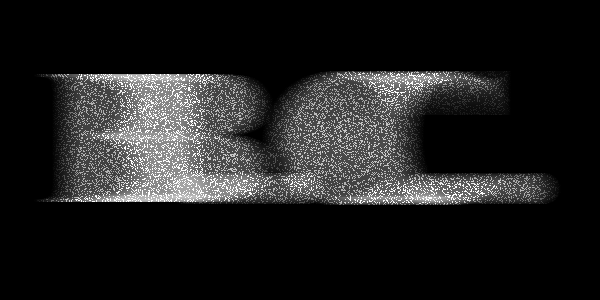
\includegraphics[width=0.43\textwidth]{BCnoisy}};}\qquad 
\tikz[remember picture]{\node(e){
\includegraphics[width=0.43\textwidth]{BC}};}
\qquad
\vskip 10pt
\tikz[remember picture]{\node(f){constant speed horizontal motion};}
  
  \tikz[remember picture,overlay]{
    \draw[->] (a.south) to (d.north) ;
    \draw[->] (c.south) to (e.north) ;
    \draw[->] (b.south) to (f.north) ;
    }
\end{frame}

\begin{frame}{Fredholm Integral Equations of the First Kind (FIE)}

\begin{itemize}
\item Applications: PDEs, indirect density estimation, signal reconstruction, causal inference, ...
\item Ill posed inverse problems
\item Solution methods often require discretisation/strong assumptions on $\rho$
\end{itemize}
\end{frame}

\begin{frame}{FIE - Solution method}
\begin{equation*}
\mu(dy) = \int \rho(dx) K(x,dy),
\end{equation*}
Take $\rho,\mu$ probability measures and $K$ a Markov transition kernel
\begin{equation*}
\rho^\star:= \text{argmin}\KL(\mu,\rho K)-\alpha\ent(\rho)
\end{equation*}
for some $\alpha>0$.
\pause

How?
\begin{align*}
\text{minimisation}\longrightarrow \text{PDE}\longrightarrow \text{SDE}
\end{align*}
\end{frame}

\begin{frame}{Gradient Flows}
\centering
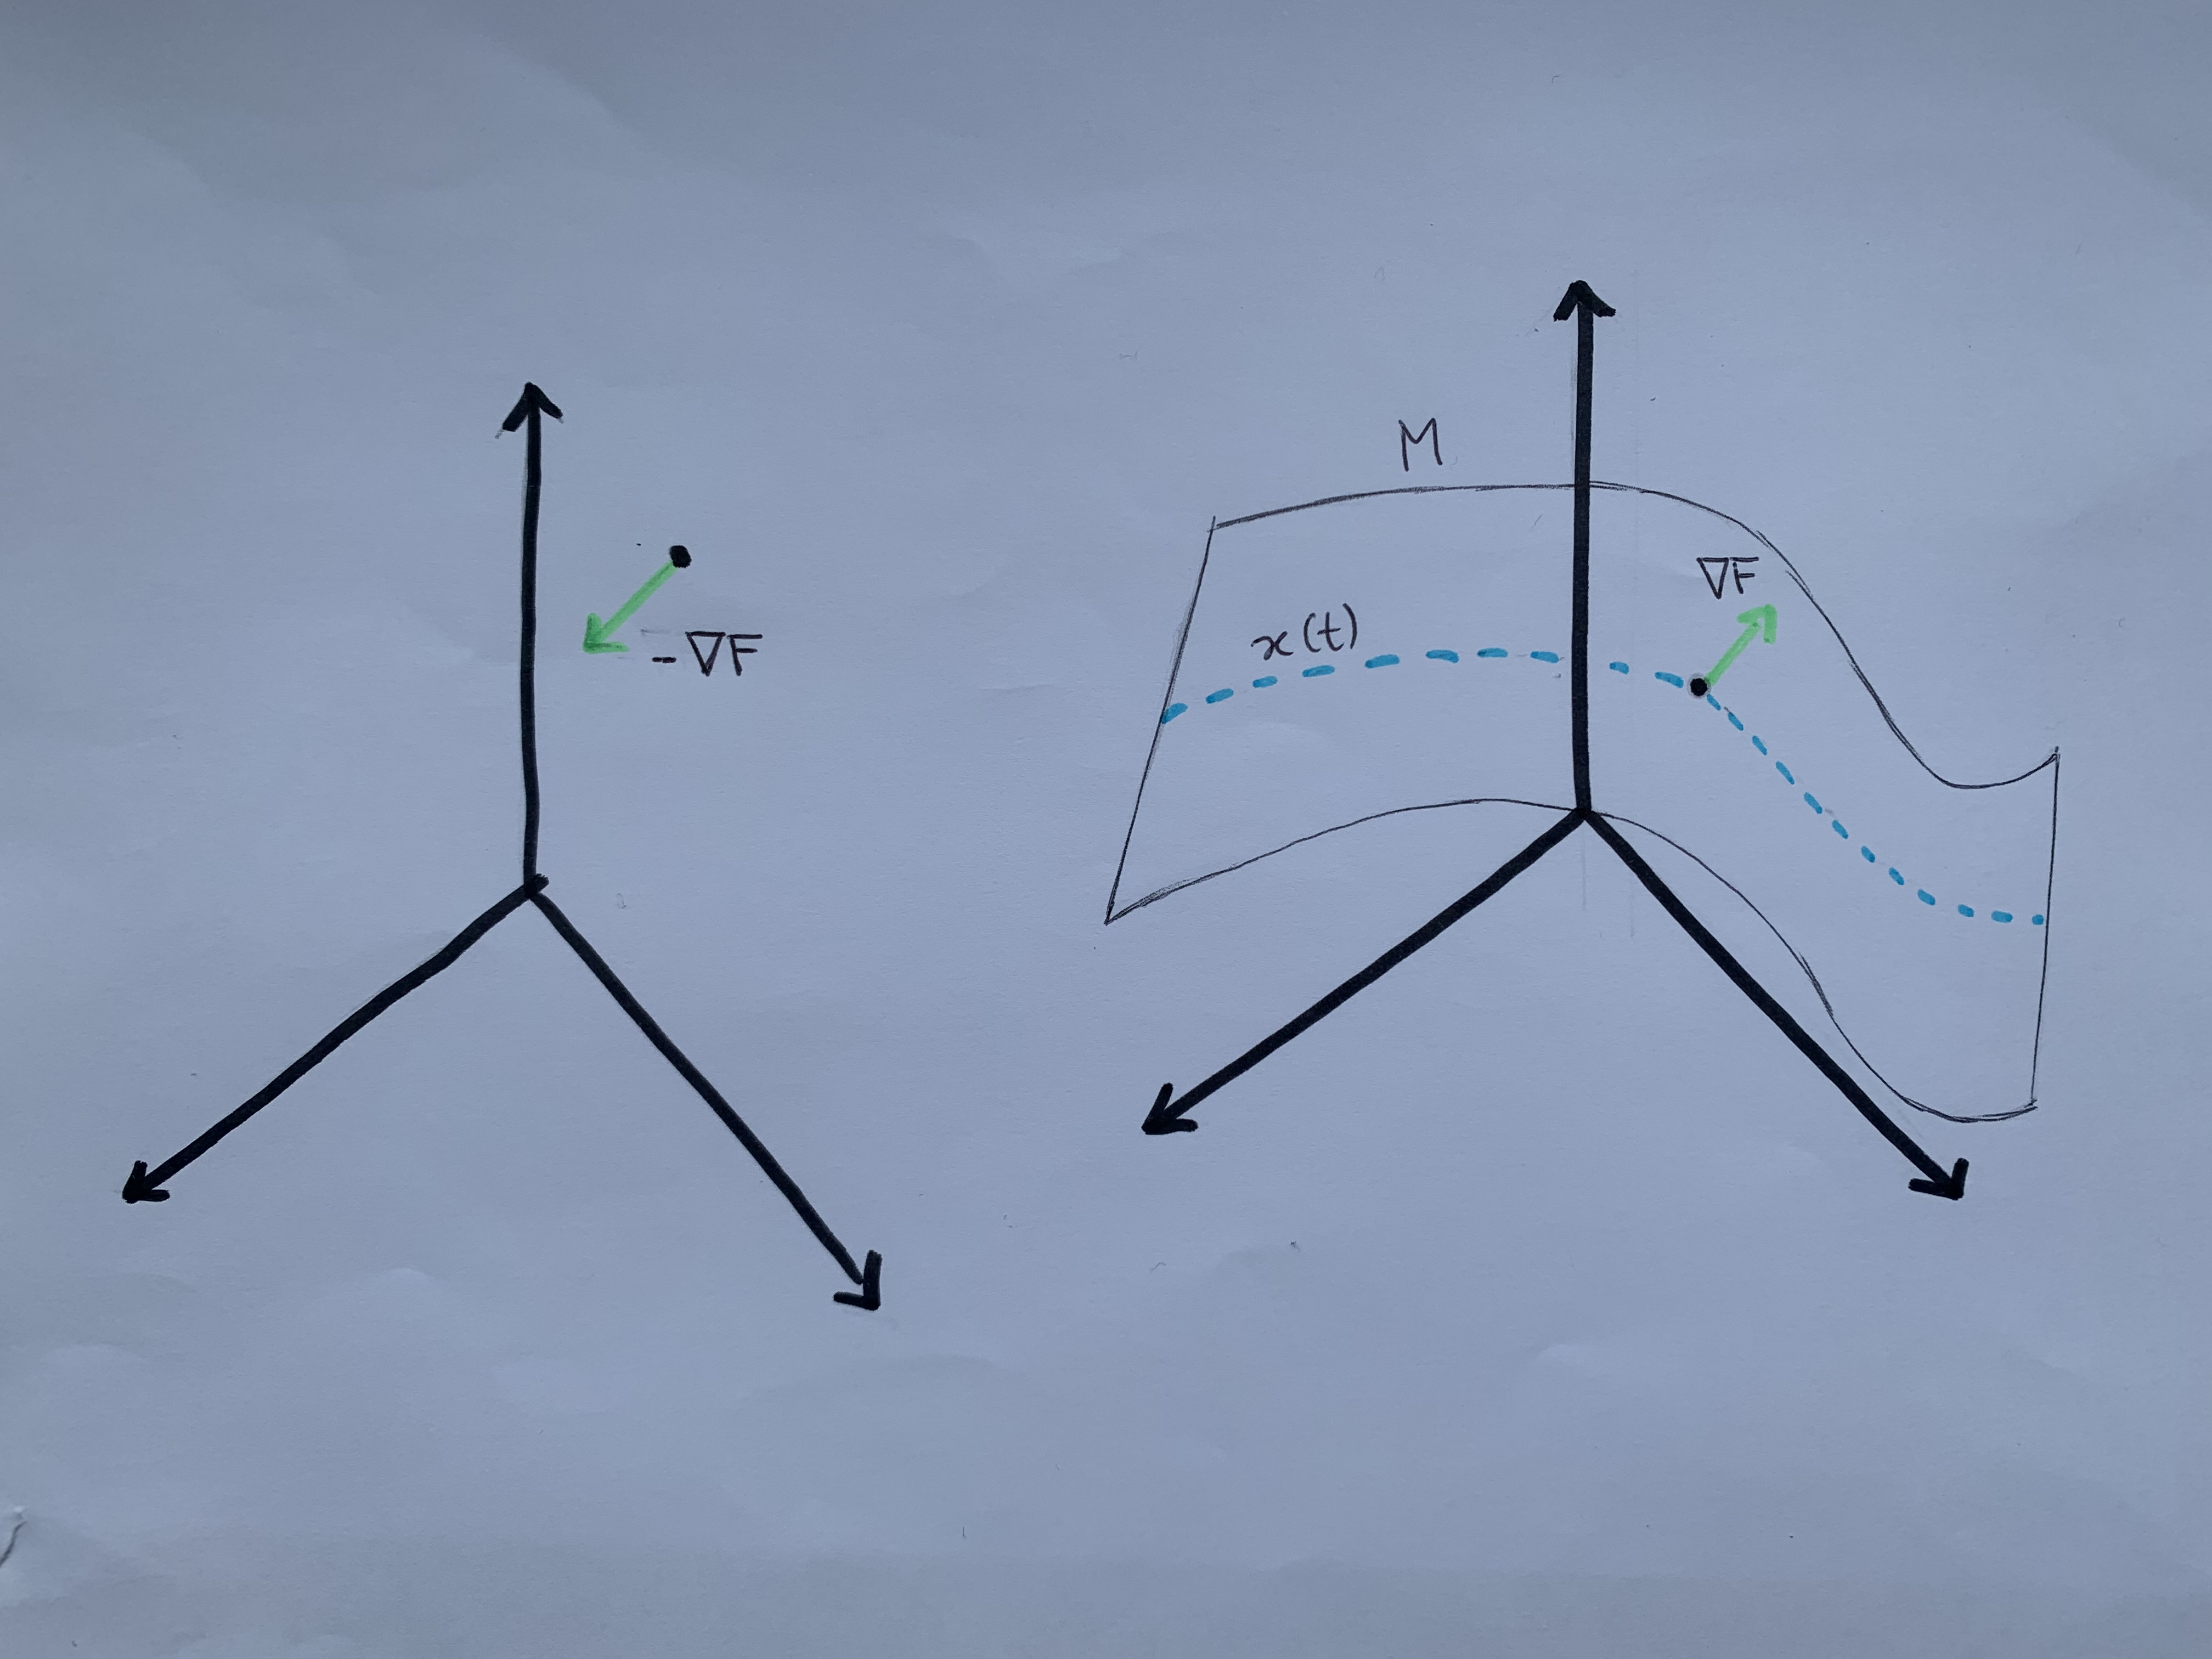
\includegraphics[width=0.7\textwidth]{gf}
\begin{align*}
x^\prime(t)=-\nabla F(x(t))
\end{align*}
\end{frame}

\begin{frame}{Wasserstein Gradient Flows - Space}
\begin{itemize}
\item Extension of gradient flows to probability measures
\item In particular, probability measures $\mu$ with finite second moment
\begin{align*}
\int\norm{x}{2}^{2}\ d\mu(x)<\infty
\end{align*}
and absolutely continuous w.r.t. Lebesque $\mu\ll\mathcal{L}$: $\mathcal{P}_{2}^{ac}(\real^{d})$
\end{itemize}
\end{frame}

\begin{frame}{Wasserstein Gradient Flows - Distance}
2-Wasserstein distance
\begin{align*}
W_{2}(\mu,\nu):=\left(\inf_{\pi\in\Pi(\mu,\nu)}\int\norm{x-y}{2}^{2}\ d\pi(x,y)\right)^{1/2}
\end{align*}

e.g. 1D densities $f$ and $g(x)=f(x-h)$\footnote{Santambrogio (2017)}
\begin{figure}
\centering
\resizebox{!}{0.35\textwidth}{%
\begin{tikzpicture}[every node/.append style={font=\normalsize}]
\node (img1) {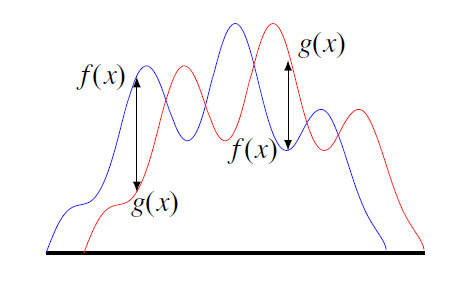
\includegraphics[width=0.4\textwidth]{lp}};
\node[below=of img1, node distance = 0, yshift = 1cm] {$\mathbb{L}_2$};
\node[right=of img1, xshift= -0.5cm] (img2) {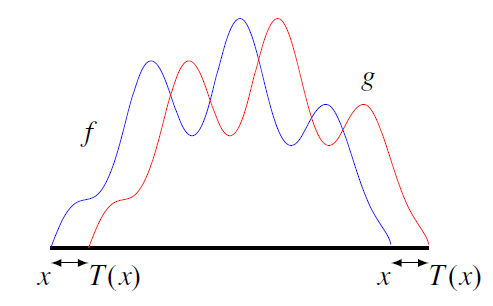
\includegraphics[width=0.4\textwidth]{wasserstein}};
\node[below=of img2, node distance = 0, yshift = 1cm] {$W_2$};
\end{tikzpicture}
}
\end{figure}

\end{frame}


\begin{frame}{Wasserstein Gradient Flows - Curves}
Curves in $\left(\mathcal{P}_{2}^{ac}(\real^{d}), W_2\right)$ are geodesics
\begin{align*}
\mu_s=((1-s)Id+st_{\mu}^{\nu})_{\#}\mu
\end{align*}
where $T_{\#}\mu$ denotes the push-forward measure $T_{\#}\mu(A)=\mu(T^{-1}(A))$
and $t_{\mu}^{\nu}$ is the unique optimal transport map between $\mu$ and $\nu$:
\begin{align*}
(t_{\mu}^{\nu}){\#}\mu=\nu,\qquad W_{2}(\mu,\nu)=\left(\int\norm{x-t_{\mu}^{\nu}(x)}{2}^{2}\ d\mu(x)\right)^{1/2}
\end{align*}
\end{frame}

\begin{frame}{Wasserstein Gradient Flows - PDE}

For $F:M\subset \real^d\rightarrow \real$ the gradient flow equation is
\begin{align*}
x^\prime(t)=-\nabla F(x(t)).
\end{align*}

For $F:\mathcal{P}_{2}^{ac}(\real^{d})\rightarrow \real$
we have\footnote{Jordan, Kinderlehrer, Otto (1998)}
\begin{align}
\label{eq:pde}
\partial_{t}\rho_{t}=-\nabla\cdot\left(\rho_{t}\variation{\rho_t}\right)
\end{align}
with
\begin{align*}
\variation{\rho_t}:=\lim_{\epsilon\rightarrow0}\frac{F(\rho+\epsilon\chi) - F(\rho)}{ \epsilon}.
\end{align*}
\end{frame}

\begin{frame}{When is \eqref{eq:pde} well-behaved?}
$F:\real^d\rightarrow \real$ is $\lambda$-convex if for $s\in[0, 1]$
\begin{align*}
F(sx+(1-s)y)\leq sF(x)+(1-s)F(y)-\frac {\lambda}{2}s(1-s)\norm{x-y}{2}^{2}
\end{align*}

\begin{figure}
\centering
\resizebox{!}{0.4\textwidth}{%
\begin{tikzpicture}[every node/.append style={font=\normalsize}]
\node (img1) {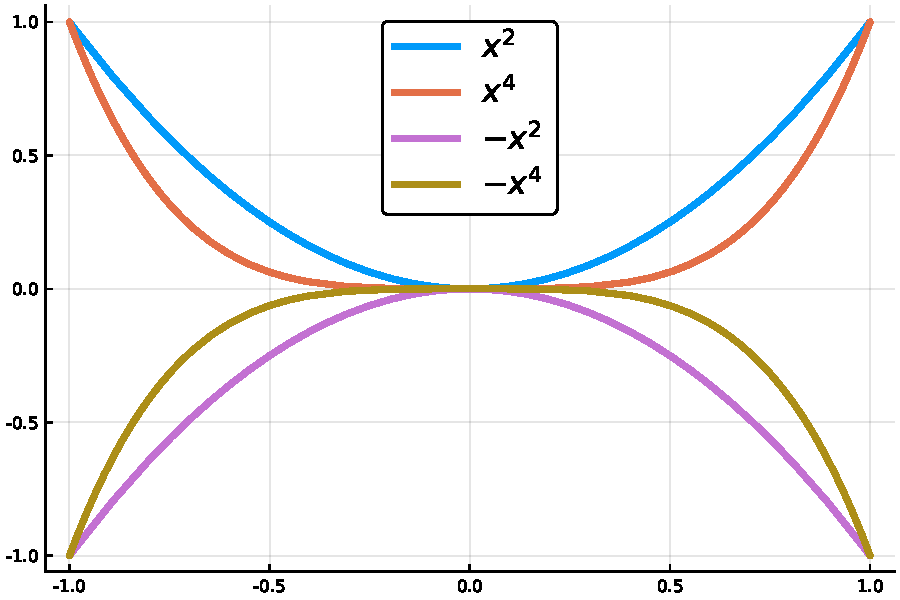
\includegraphics[width=0.4\textwidth]{lambda_convexity}};
\end{tikzpicture}
}
\end{figure}
\end{frame}


\begin{frame}{When is \eqref{eq:pde} well-behaved?}
We need:
\begin{itemize}
\item $F$ continuous, $F(\rho)<+\infty$ for some $\rho$
\item $F$ $\lambda-$geodesically convex w.r.t. $W_2$ with $\lambda\geq0$
%\begin{align*}
%F\left(((1-s)Id+st_{\mu}^{\nu})_{\#}\mu\right)\leq(1-s)F(\mu)+sF(\nu)-\frac{\lambda}{2}s(1-s)W_{2}^{2}(\nu,\mu)
%\end{align*}
\item $F$ is coercive: exists $r>0$ s.t.
\begin{align*}
\inf\left\lbrace F(\rho): \rho\in\mathcal{P}_{2}^{ac}(\real^{d}), \ \int\norm{x}{2}^{2}\ d\rho(x)\leq r\right\rbrace>-\infty
\end{align*}
\end{itemize}
\end{frame}

\begin{frame}{Then...}
The gradient flow PDE \eqref{eq:pde} has a unique solution for a given initial condition $\rho_0$.

\vspace{5mm}

For two initial conditions $\rho_0^1, \rho_0^2$ we have the estimate
\begin{align*}
W_{2}(\rho_{t}^{1},\rho_{t}^{2})\leq e^{-\lambda t}W_{2}(\rho_{0}^{1},\rho_{0}^{2}).
\end{align*}
\end{frame}

\begin{frame}{Gradient Flow for FIE - Assumptions}
\begin{equation*}
\mu(dy) = \int_{\X} \rho(dx) K(x,dy)\qquad \forall y \in \Y, 
\end{equation*}


\begin{enumerate}
    \item $\X, \Y$ subsets of some Euclidean spaces with Borel $\sigma$-algebras; 
    \item $\mu, \rho \in\mathcal{P}_2^{ac}(\X)$;
    \item $K$ bounded and bounded away from 0, Lipschitz continuous with Lipschitz continuous gradient and for fixed $y\in\Y$, $\lambda$-concave in $x$ for some $\lambda>0$.
\end{enumerate}
\end{frame}

\begin{frame}{Gradient Flow for FIE}
\begin{equation*}
F(\rho) := \KL(\mu,\rho K)-\alpha\ent(\rho)
\end{equation*}
is continuous, coercive and $\lambda$ geodesically convex with $\lambda=0$ and has first variation
\begin{equation*}
\variation{\rho}\left(x\right)=-\int\mu\left(dy\right)\frac{K(x,y)}{\rho K(y)}+\alpha\left(1+\log\rho\left(x\right)\right).
\end{equation*}

\vspace{5mm}

\arrowright the gradient flow exist and is unique for each initial condition $\rho_0$
\end{frame}

\begin{frame}{Gradient Flow for FIE - PDE}
\begin{align*}
\partial_{t}\rho_{t}&=\nabla\cdot\left(\rho_{t}\nabla\variation{\rho_{t}}\right)\\
&=\nabla\cdot\left(\rho_t\left[-\int\mu\left(dy\right)\frac{\nabla K(x,y)}{\rho K(y)}+\alpha\nabla\log\rho\left(x\right)\right]\right)\\
&=-\nabla\cdot\left(\rho_{t}\int\mu\left(dy\right)\frac{\nabla K(x,y)}{\rho_{t}K(y)}\right)+\alpha\triangle\rho_{t}
\end{align*}
is a Fokker-Plank equation with corresponding SDE...
\end{frame}

\begin{frame}{Gradient Flow for FIE - SDE}
\begin{align*}
dX_{t}=\int\mu\left(dy\right)\frac{\nabla K(X_{t},y)}{\rho_{t}K(y)}dt+\sqrt{2\alpha}dW_{t},\quad X_{0}\sim\rho_{0}
\end{align*}

\begin{itemize}
\item McKean-Vlasov SDE
\item a strong solution exists and is unique
\item requires discretisation in time and space
\end{itemize}
\end{frame}

\begin{frame}{SDE - Implementation}
\begin{itemize}
\item discretisation in space: take $N$ copies of the SDE and use the resulting empirical measure instead of $\rho_t$
\begin{align*}
dX_{t}^{i}=\int\mu\left(dy\right)\frac{\nabla K(X_{t}^{i},y)}{\rho_{t}^{N}K(y)}dt+\sqrt{2\alpha}dW_{t}^{i},\quad\rho_{t}^{N}=\frac{1}{N}\sum_{i=1}^{N}\delta_{X_{t}^{i}}
\end{align*}
\item discretisation in time: Euler scheme
\begin{align*}
X_{n+1}^{i}& =X_{n}^{i}+\int\mu\left(dy\right)\frac{\nabla K(X_{n}^{i},y)}{\rho_{n}^{N}K(y)}\Delta t+\sqrt{2\alpha}\Delta W^{i}_n,\\
&\rho_{n}^{N}=\frac{1}{N}\sum_{i=1}^{N}\delta_{X_{n}^{i}}
\end{align*}
\end{itemize}
\end{frame}

\begin{frame}{Toy Example}
\begin{equation*}
\mu(dy) = \int_{\X} \rho(dx) K(x, dy), 
\end{equation*}
with 
\begin{align*}
\mu(y)&=\N(y;m,\sigma_{\mu}^{2}:=\sigma_{K}^{2}+\sigma_{\rho}^{2})\\
K(x,y)&=\N(y;x,\sigma_{K}^{2})\\
\rho(x)&=\N(x;m,\sigma_{\rho}^{2}).
\end{align*}

The unique minimiser of $E$ is
\begin{align*}
\rho_\alpha(x)&=\N(x;m,\sigma_{\alpha}^{2})
\end{align*}
for $\alpha\in[0, 1)$.
\end{frame}
\begin{frame}
A number of quantities need to be specified
\begin{itemize}
\item regularisation: $\alpha$
\item gradient flow set up: $\rho_0$
\item numerical approximation of SDE: $N$ (500/1000), $\Delta t$ ($10^{-3}$ is enough)
\end{itemize}

And, how does it compare to other methods?
\end{frame}

\begin{frame}{$\rho_0$}
\begin{figure}
\centering
\resizebox{!}{0.4\textwidth}{%
\begin{tikzpicture}[every node/.append style={font=\normalsize}]
\node (img1) {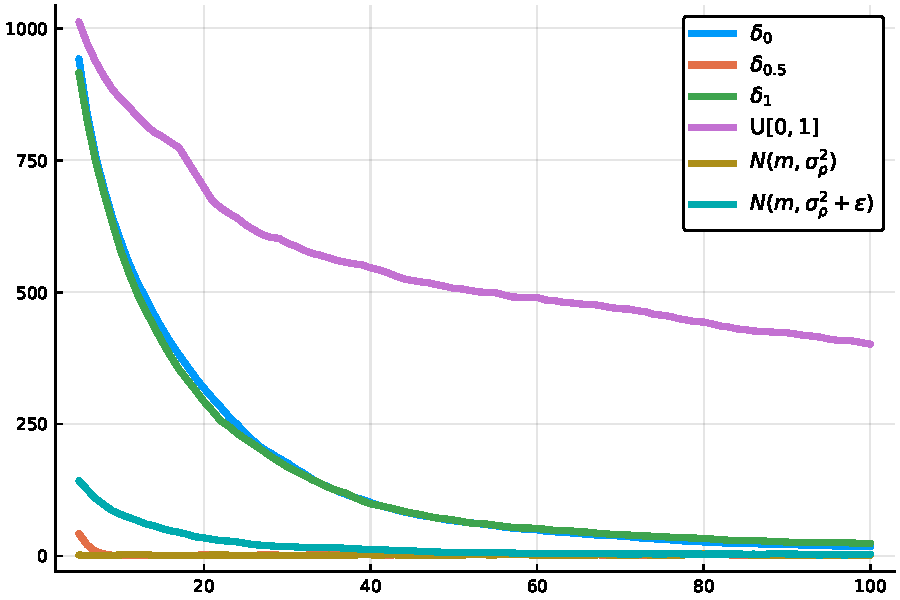
\includegraphics[width=0.5\textwidth]{initial_distribution_E}};
\node[above=of img1, node distance = 0, yshift = -1cm] {100 iterations};
\node[below=of img1, node distance = 0, yshift = 1cm] {Iteration};
  \node[left=of img1, node distance = 0, rotate=90, anchor = center, yshift = -0.9cm] {$E(\hat{\rho})$};
\node[right=of img1, xshift= -0.5cm] (img2) {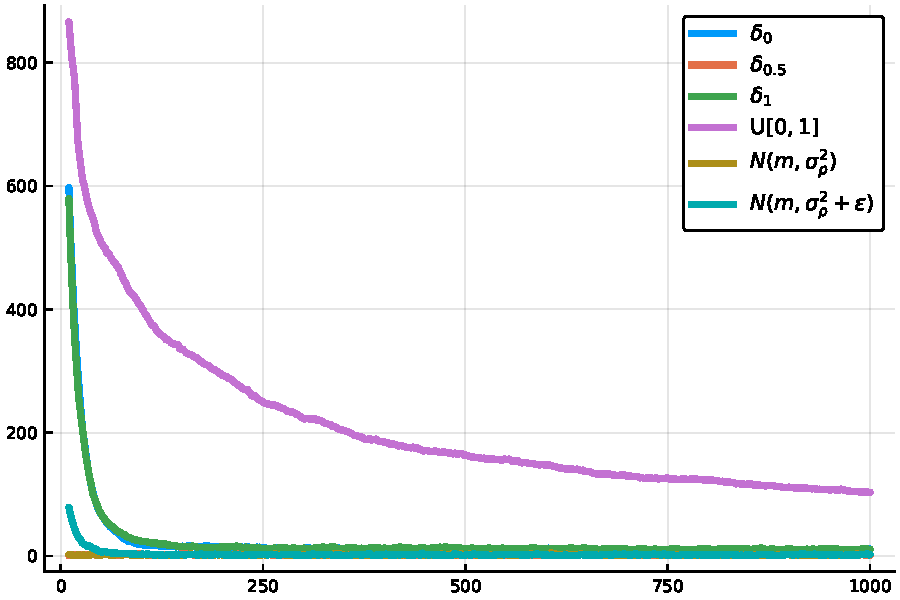
\includegraphics[width=0.5\textwidth]{initial_distribution_E_1000iter}};
\node[above=of img2, node distance = 0, yshift = -1cm] {1000 iterations};
\node[below=of img2, node distance = 0, yshift = 1cm] {Iteration};
  \node[left=of img2, node distance = 0, rotate=90, anchor = center, yshift = -0.9cm] {$E(\hat{\rho})$};
\end{tikzpicture}
}
\end{figure}
\end{frame}

\begin{frame}{$\alpha$}
\begin{figure}
\centering
\resizebox{!}{0.4\textwidth}{%
\begin{tikzpicture}[every node/.append style={font=\normalsize}]
\node (img1) {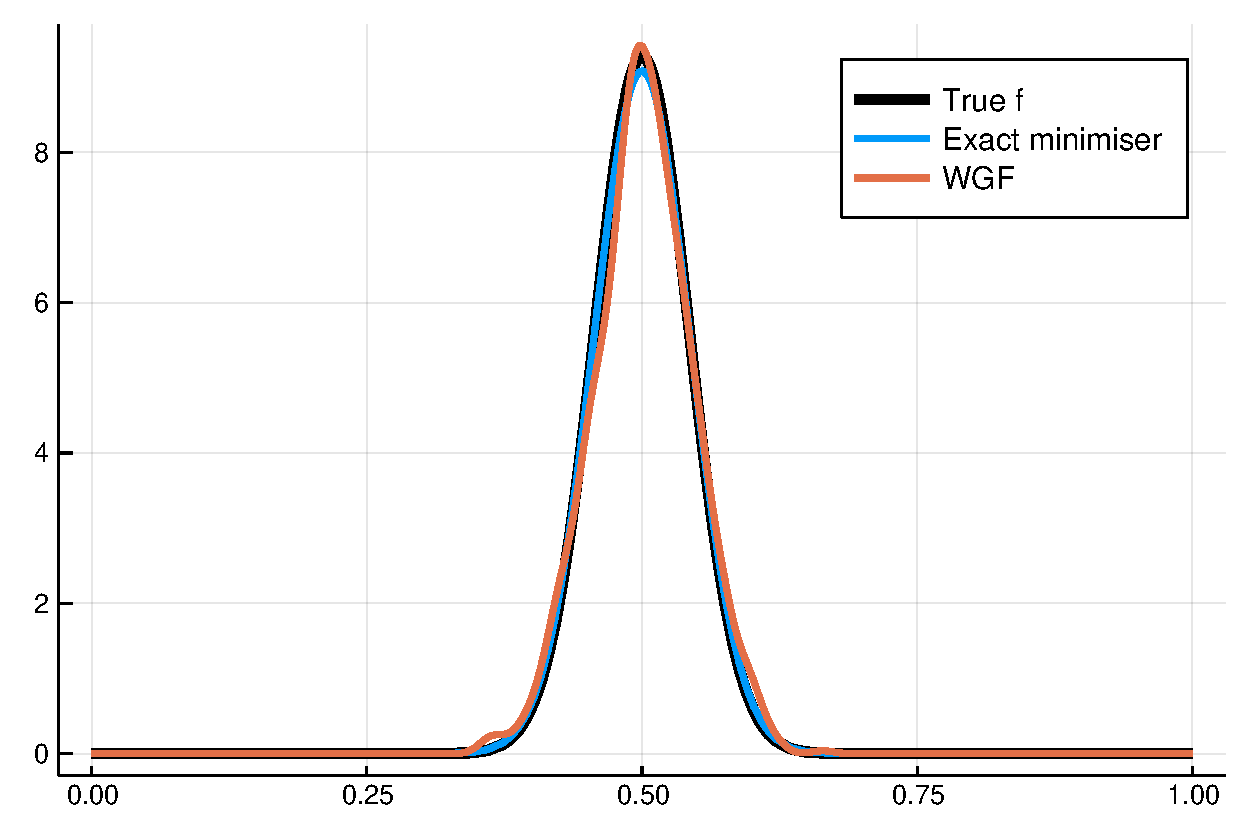
\includegraphics[width=0.5\textwidth]{at_alpha_small}};
\node[above=of img1, node distance = 0, yshift = -1cm] {$\alpha=0.01$};
\node[below=of img1, node distance = 0, yshift = 1cm] {$x$};
  \node[left=of img1, node distance = 0, rotate=90, anchor = center, yshift = -0.9cm] {$\rho(x)$};
\node[right=of img1, xshift= -0.5cm] (img2) {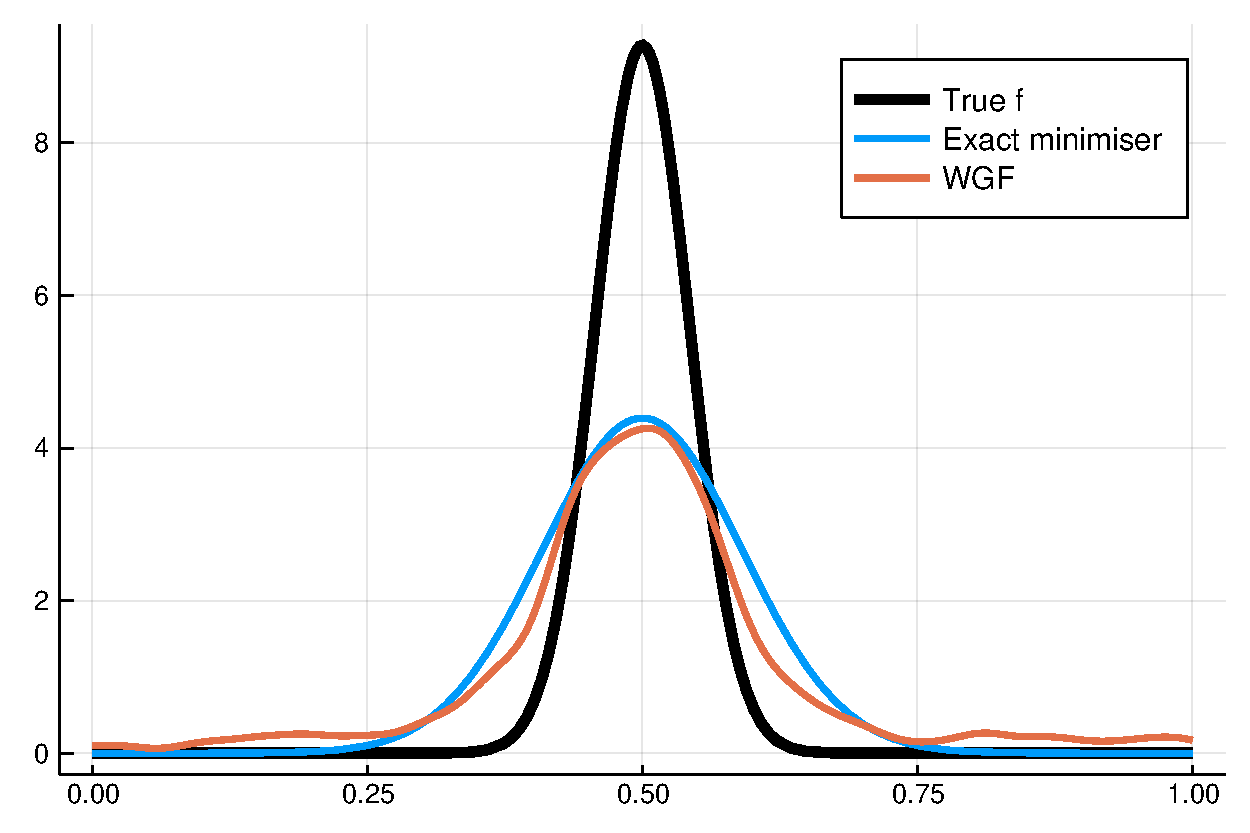
\includegraphics[width=0.5\textwidth]{at_alpha_large}};
\node[above=of img2, node distance = 0, yshift = -1cm] {$\alpha=0.5$};
\node[below=of img2, node distance = 0, yshift = 1cm] {$x$};
  \node[left=of img2, node distance = 0, rotate=90, anchor = center, yshift = -0.9cm] {$\rho(x)$};
\end{tikzpicture}
}
\end{figure}
\end{frame}

\begin{frame}{Comparison}

\end{frame}
%\begin{frame}{A second Toy Example}
%
%\centering
%\resizebox{!}{0.45\textwidth}{%
%\begin{tikzpicture}[every node/.append style={font=\normalsize}]
%%\node (img1) {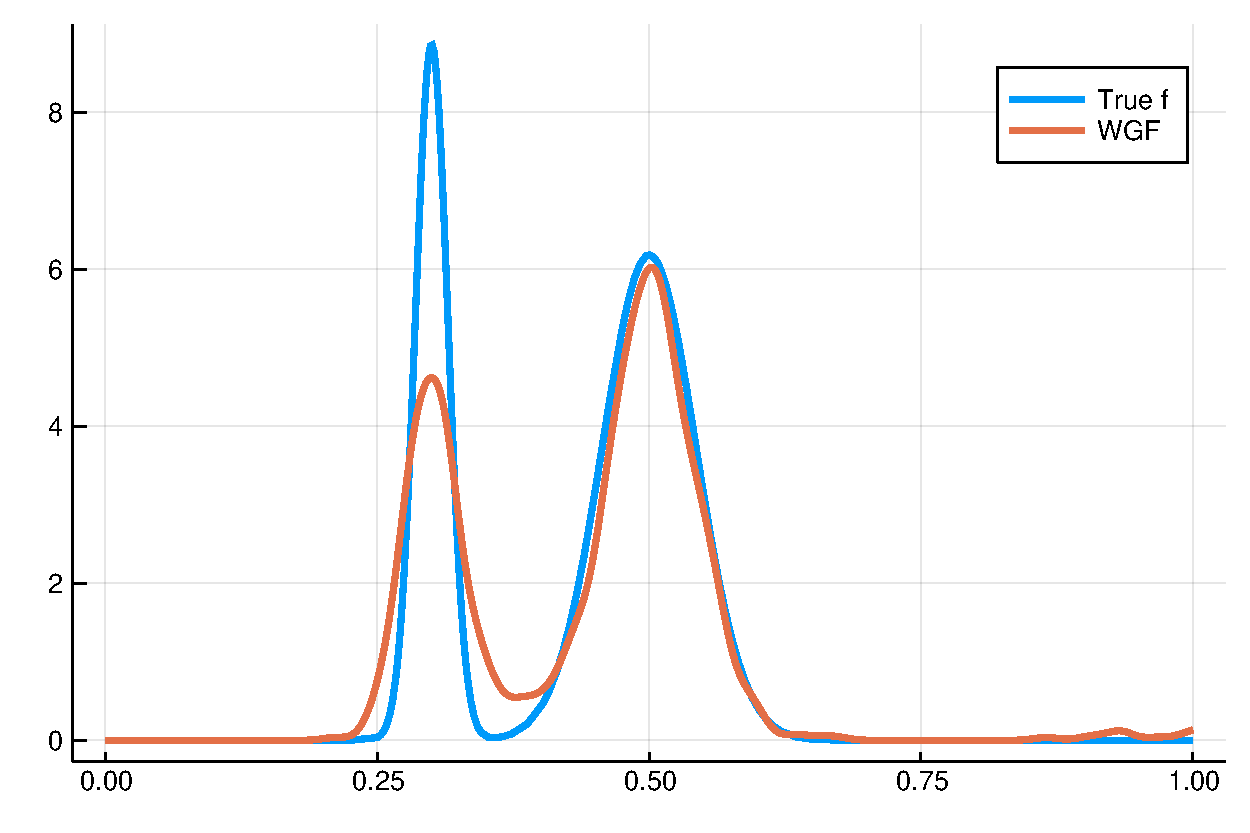
\includegraphics[width=0.4\textwidth]{Images/mixture}};
%%\node[below=of img1, node distance = 0, yshift = 1cm] {$x$};
%%  \node[left=of img1, node distance = 0, rotate=90, anchor = center, yshift = -0.9cm] {$\rho(x)$};
%\node[right=of img1, xshift= -0.5cm] (img2) {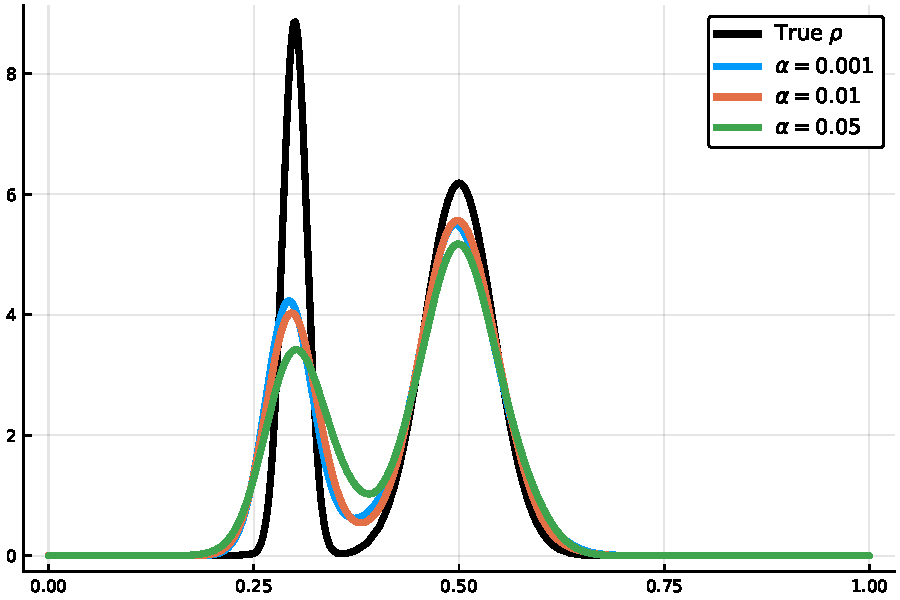
\includegraphics[width=0.45\textwidth]{Images/mixture_alpha}};
%\node[below=of img2, node distance = 0, yshift = 1cm] {$x$};
%  \node[left=of img2, node distance = 0, rotate=90, anchor = center, yshift = -0.9cm] {$\rho(x)$};
%\end{tikzpicture}
%}
%\end{frame}

\begin{frame}{PET}
The reconstruction of a cross-section of the brain (a) from the data image provided by PET scanners (b) is described by a 2D Fredholm integral equation of the first kind.

\begin{figure}
\setcounter{subfigure}{0}
\centering
\subfloat[128-pixels Shepp-Logan phantom \label{fig:phantom}]{

\includegraphics[height=0.45\textheight]{phantom}}\qquad
\subfloat[Sinogram + noise \label{fig:sinogram}]{
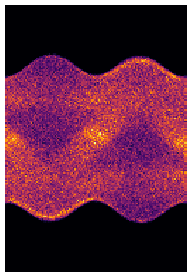
\includegraphics[height=0.45\textheight]{sinogram}}
\end{figure}
\end{frame}
\end{document}